
Para realizar la simulaci\'on se dispuso la estructura cristalina de ambos 
materiales en varios arreglos antiferromagn\'eticos. Esto se logr\'o colocando 
los espines de los \'atomos de hierro y cromo del $BiFeO_{3}$ y $YCrO_{3}$ 
respectivamente, en direcciones paralelas y antiparalelas entre ellos de 
acuerdo a los tipos de arreglos antiferromagn\'eticos escogidos. 
En el caso del $BiFeO_{3}$ se utilizaron los arreglos antiferromagn\'eticos 
tipo A y G, los cuales se pueden observar en forma esquem\'atica en la figura 
\ref{arreglos_BFO}.

\begin{figure}[H]
	\centering
	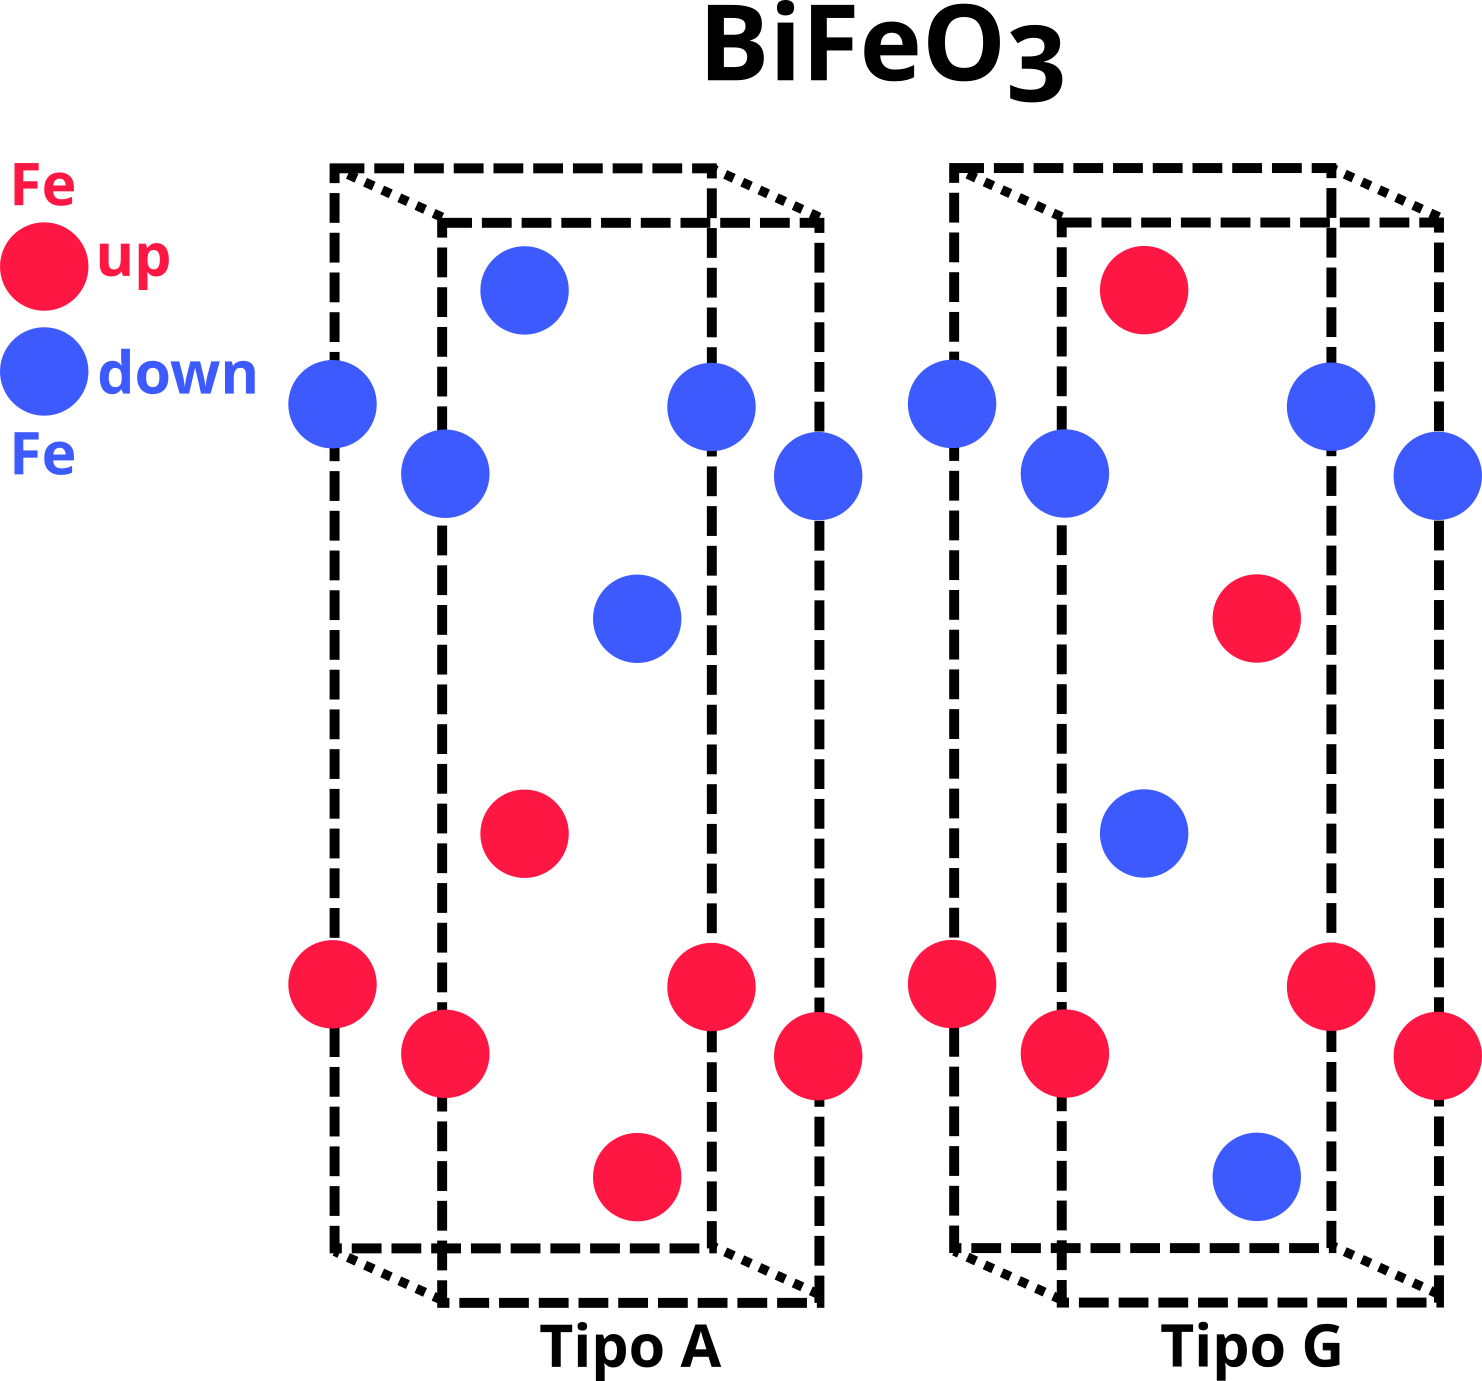
\includegraphics[width=0.5\textwidth]{contenido/calculos_computacionales/arreglos_antiferromagneticos/img_arreglos/BFO_unido.png}
	\caption[Arreglos antiferromagn\'eticos $BiFeO_{3}$]{Arreglos 
		antiferromagn\'eticos para el $BiFeO_{3}$ se muestran solo los \'atomos 
		de hierro por claridad.}
	\label{arreglos_BFO}
\end{figure}

\noindent En el caso del $YCrO_{3}$ se utilizaron los arreglos 
antiferromagn\'eticos tipo 
A, C y G, los cuales se pueden observar en forma esquem\'atica en la figura 
\ref{arreglos_YCO}.

\begin{figure}[H]
	\centering
	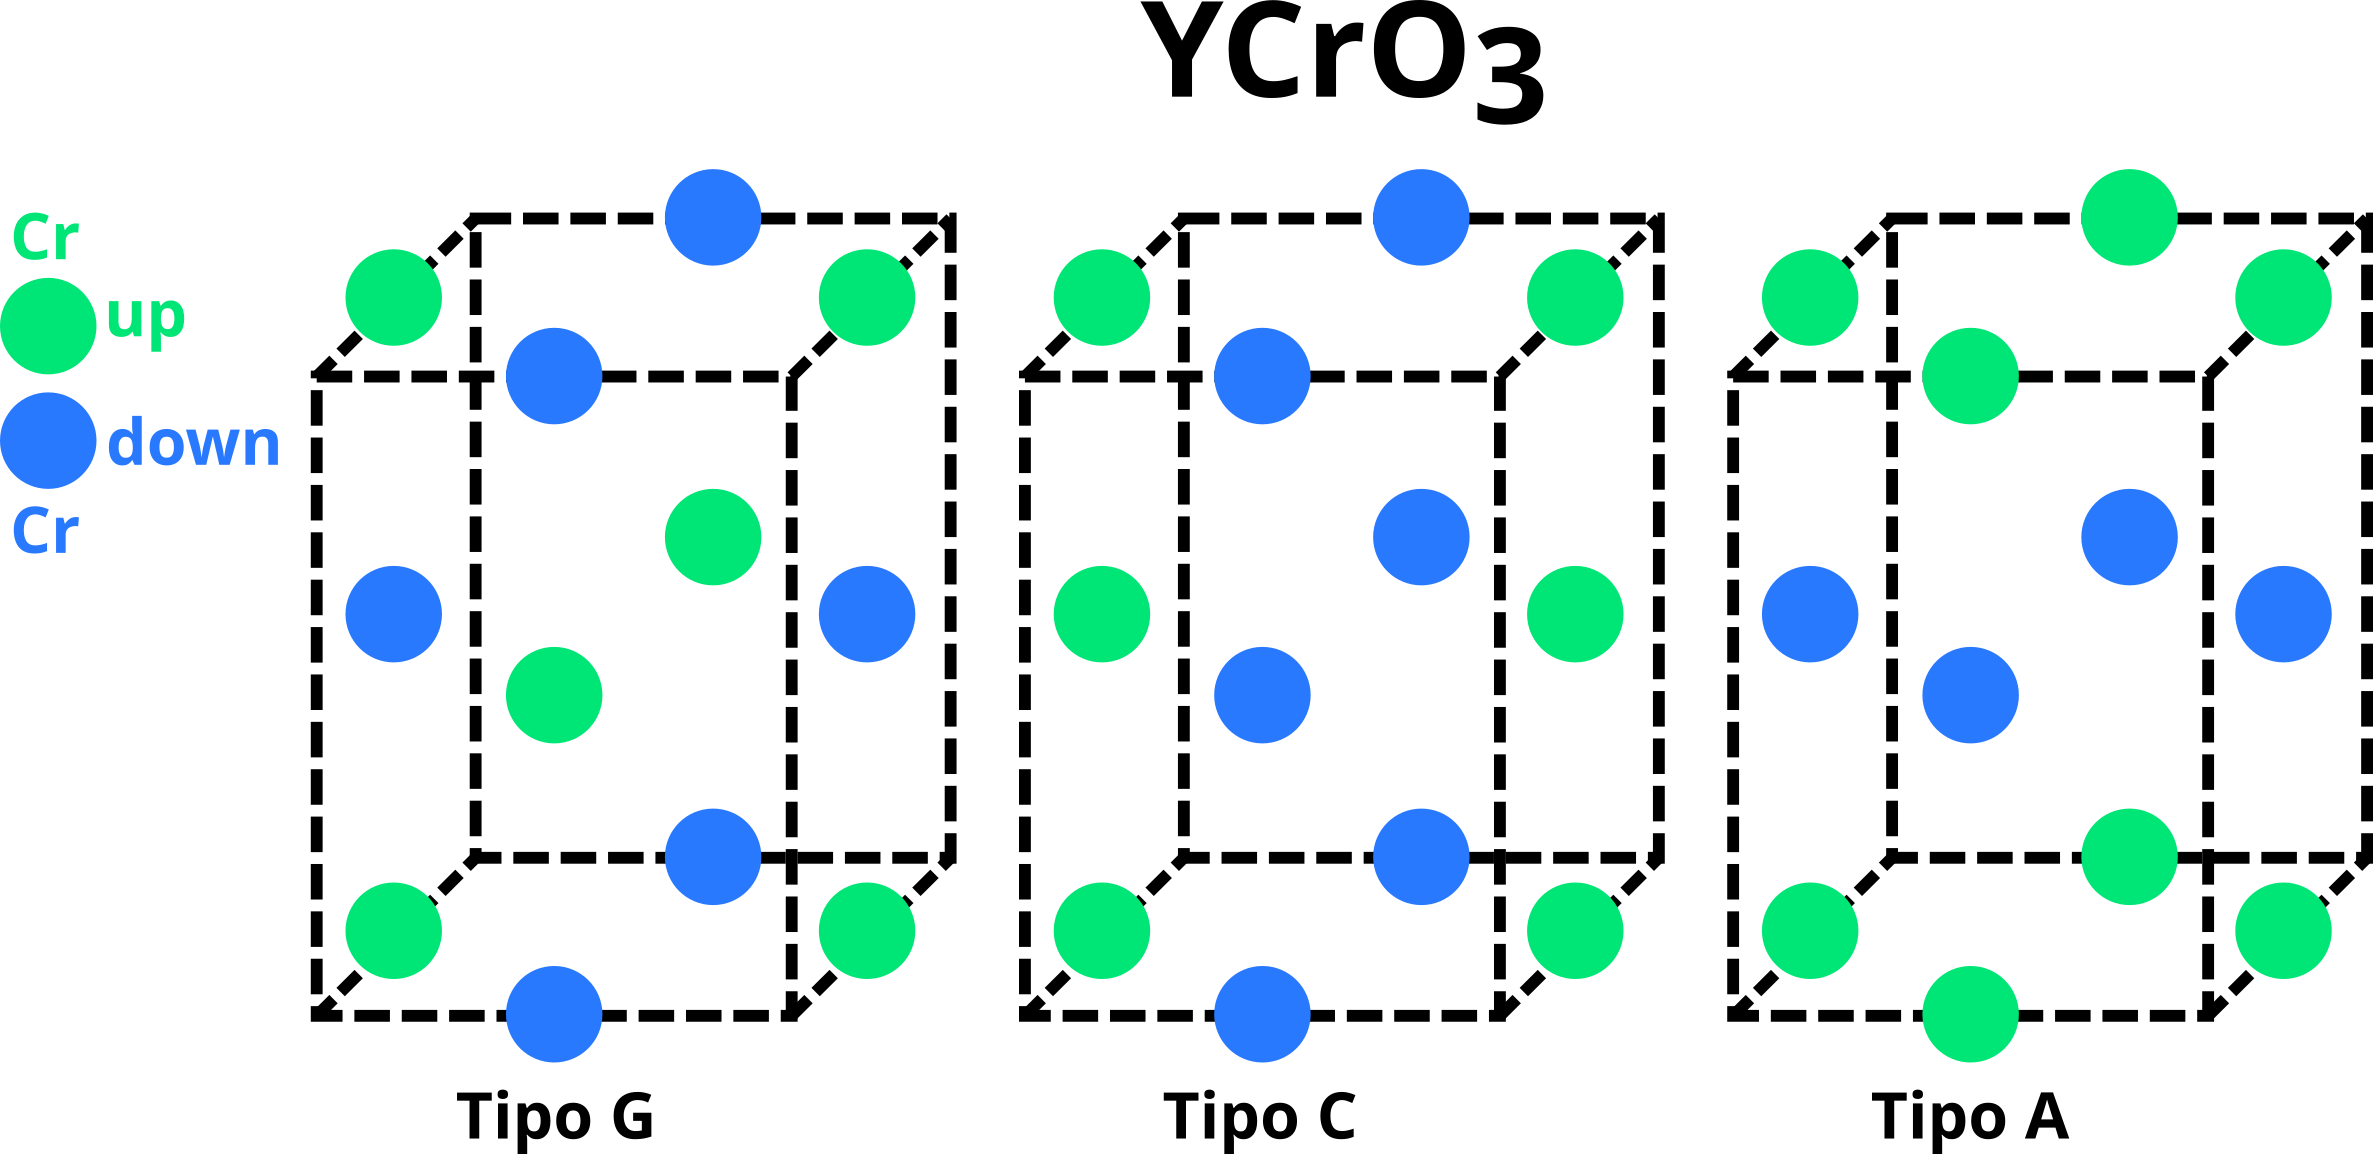
\includegraphics[width=0.6\textwidth]{contenido/calculos_computacionales/arreglos_antiferromagneticos/img_arreglos/YCO_unido.png}
	\caption[Arreglos antiferromagn\'eticos $BiFeO_{3}$]{Arreglos 
		antiferromagn\'eticos para el $YCrO_{3}$ se muestran solo los \'atomos 
		de cromo por claridad.}
	\label{arreglos_YCO}
\end{figure}